\chapter{改进OpenShift Origin平台调度策略}
\label{cha:openshift}
Kubernetes作为OpenShift Origin容器云平台的容器编排引擎,其默认配置的调度算法虽能满足大部分用户需求,但其算法较为简单,集群资源利用率较低,也不能满足用户的在特定场景下的调度。本章在深入分析默认调度算法后,提出设计了一种新的基于多维资源空闲率权重的评价函数和调度方案MRWS (Multidimensional Resource WeightSscheduling)。

\section{优化Kubernetes调度流程}
Kubernetes调度算法分为预选和优选两阶段,在预选阶段过滤掉不满足需求的节点,优选阶段对剩余节点评分,选择评分最高的节点作为调度目标。整个调度器可以分为待调度的Pod列表、满足条件的Node列表以及调度策略三部分。用户除开发特殊的调度算法外,还可以针对其调度流程进行适当的优化。

\subsection{Default调度算法流程}
在Kubernetes默认调度流程,预选阶段解决节点过滤,优选阶段解决最优节点选择问题,用户可以对两个阶段进行简单的配置,调度器将根据用户指定的预选和优选规则进行过滤和评分计算,最终输出满足条件的Node和Pod绑定策略,将Pod调度到Node节点上,针对两阶段的规则,下面做详细的介绍。
\begin{figure}[H] % use float package if you want it here
	\centering
	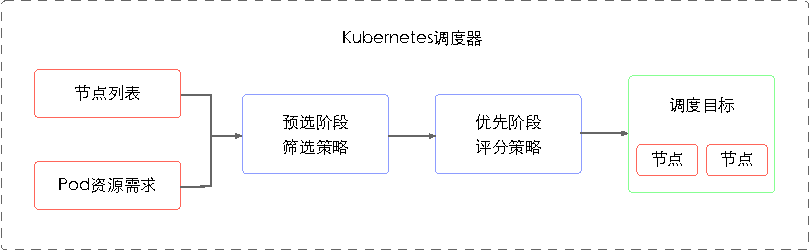
\includegraphics{scheduler-default}
	\caption{Default调度算法流程}
	\label{fig:xfig1}
\end{figure}
Predicates策略过滤掉不满足Pod需求的节点,主要依据磁盘卷是否冲突、端口冲突、资源容量、节点检测、服务占用、亲和性筛选等条件。1.7版本的筛选条件主要如下,新的版本Kubernetes还在不断完善和更新:
\begin{enumerate}[(1)]
	\item NoDiskConflict:检测卷冲突,在当前的规则中,两个不同Pod不能使用相同的卷此一旦Node上已经挂载了该卷并被某个Pod使用,则新的Pod不能再调度到该Node上,否则造成卷冲突。不同的系统对该冲突检测范围不同,如Google Compute Engine在只读模式下允许多个卷,Ceph RDB允许两个Pod分享部分资源,Amazon EBS禁止两个Pod挂载同一个卷。
	\item NoVolumeZoneConflict:在给定Zone限制的条件下,检测Node上部署的Pod是否存在卷冲突,当前只限定对PV(PersistantVolume)范围进行支持。
	\item PodFitsHostPorts:端口冲突和服务占用检测,需要调度的Pod内所有的容器需要的端口在Node上是否被其他Pod占用。
	\item PodFitsResources:根据Pod资源的需求检测节点空闲资源量是否满足其运行需求,主要检测CPU、内存、磁盘等资源。Kubernetes的调度是静态调度,资源的判断是根据分配的资源量而不是资源的实际使用量。
	\item HostName:检测Pod是否指定了Node节点,所有不在制定Node集合内的节点都将被过滤掉。
	\item MatchNodeSelector:检测Pod是否指定了MatchNodeSelector属性,若指定了该属性,Node的Label必须和该属性匹配。
	\item MaxEBSVolumeCount:确保挂载的EBS存储卷总合不超过设置最大值,调度器计算每个Node上直接或间接使用的全部卷总合,一旦超过最大值,Pod不能调度到该节点上。
	\item CheckNodeMemoryPressure:判断节点是否存在内存压力,若存在内存压力则标记为1,Pod只能调度到内存标记为0的节点上。
	\item CheckNodeDiskPressure:判断节点是否存在磁盘压力,若存在磁盘压力则标记为1,Pod只能调度到磁盘标记为0节点。
	\item MatchInterPodAffinity:节点的亲和性过滤,检测Pod是否和已部署的Pod存在亲和性,将有亲和性的Pod调度到相同节点。
	\item PodToleratesNodeTaints:判断将Pod调度到节点后是否满足节点容忍的条件,相同的Pod副本为了满足容灾性,一般部署到不同的Node甚至是不同的机架和数据中心。
\end{enumerate}
此外、还有转为Google Compute Engine和Amazon EBS配置的MaxGCEPDVolumeCount、MaxAzureDiskVolumeCount卷检测条件,检测节点上挂载的卷容量总合是否超过设定的最大值。

Priorities阶段根据一定的评分算法对预选出来的节点列表进行综合评分,评分依据主要包括资源空闲量、资源消耗平衡性、Pod亲和性、Pod与节点的匹配度等因素。Kubernetes使用优先函数集合进行0-10对节点进行评分,最终计算评分总合,评分越高表明Pod调度到该节点越适合,同时还可以为每一个函数设置一个权重值,主要的评分函数如下:
\begin{enumerate}[(1)]
	\item LeastRequestedPriority:根据资源空闲率计算节点得分,即节点的空闲资源与节点资源总量的比值((节点资源总量-节点上Pod的资源和-新Pod的需求)/总容量)来计算。设置CPU和内存具有相同权重,都设置为0.5,资源空闲率越大,剩余资源越多,节点的评分就越高。
	\item BalancedResourceAllocation:该函数必须联合LeastRequestedPriority一起使用,用于平衡各项资源的使用率,资源使用越均衡,节点的评分越高。Kubernetes主要对内存和CPU资源消耗进行平衡,由两者的“距离”决定分值大小,即使用10-abs(CPU空闲率-内存空闲率)*10进行计算。
	\item SelectorSpreadPriority:为了更好应对容灾和宕机风险,同属Service、Replication Controller下的Pod尽可能分散部署到不同的Node上。对于指定Zone的Pod,也要尽量分散到不同区域的主机。调度器统计各Node上相同Service、Replication Controller下的Pod,Node上Pod数量越少,评分越高。
	\item NodeAffinityPriority:设置调度器的亲和性机制,主要对节点进行精确匹配。有两种选择器匹配模式,选择器“hard"模式下设置的NodeSelector必须和节点的Label匹配,保证选择的Node是完全满足需求规则的,”soft"模式下不能完全保证百分百的匹配,但会尽量满足规则要求
	\item ImageLocalityPriority:为避免镜像的重复下载对网络和磁盘资源的重复消耗,该函数根据Pod中运行容器需要的镜像对节点进行评分,节点上存在的镜像越多,该节点评分越高。若该节点上没有所需的镜像,评分为0,镜像评分的权重可以根据镜像大小按比例决定。
	\item MostRequestedPriority:和LeastRequestedPriority相反,两者使用一个来计算评分。该函数确保使用资源越多的节点,评分越高,目的在于使用更少的服务器提供服务,节约集群资源,提升资源利用率。
	\item TaintTolerationPriority:容忍性评分函数,匹配Pod的TolerationList与节点Taint,匹配项越多,该节点的容忍性越好,从而评分越高。
	\item InterPodAffinityPriority:用于迭代WeightedPodAffinityTerm的元素计算和,若该节点同时满足亲和性设置,则将该评分加入节点的整体评分中。
	\item NodePreferAvoidPodsPriority:根据节点是否设置Anotation属性进行评分,没有设置该属性则评分为10,设置该属性并且调度的Pod正好是副本,则该节点评分为0,目的在于避免相同副本调度到同一节点。
\end{enumerate}

优先调度模块定义了一个评分函数集合,各评分函数的权重可以指定,用户根据调度依据的重要程度给各函数赋予不同的权重值,最终所有函数的评分总合就是该节点的最终得分,选择评分最高的节点作为Pod的调度目标。

\subsection{MRWS算法调度流程}
Kubernetes调度系统的Default算法核心在于优选阶段的评分函数,调度策略根据节点评分高低做出调度决策。在所有的评分函数中,除一些特殊的调度规则外,如节点亲和性、节点容忍度、节点上的镜像文件等,最为重要的是根据资源空闲率做出评分的LeastRequestedPriority和资源使用平衡性做出评分的BalancedResourceAllocation函数。这两个函数是整个评分函数集合中的核心,在其他外在规则相同的条件下,直接决定节点的评分高低。但是,这两个评分函数仅考虑了内存和CPU的空闲率和消耗平衡性,这种评分会造成节点其他维度资源消耗不均,如I/O、带宽、节点上运行的Pod数量等,一旦某个维度的资源过载,节点将不能部署更多的Pod,造成集群资源利用率低下。因此,新的调度算法MRWS将更多关注于集群CPU、内存、磁盘、网络带宽以及节点运行Pod数量的均衡性,提升集群的负载均衡和资源利用率。
\begin{figure}[H] % use float package if you want it here
	\centering
	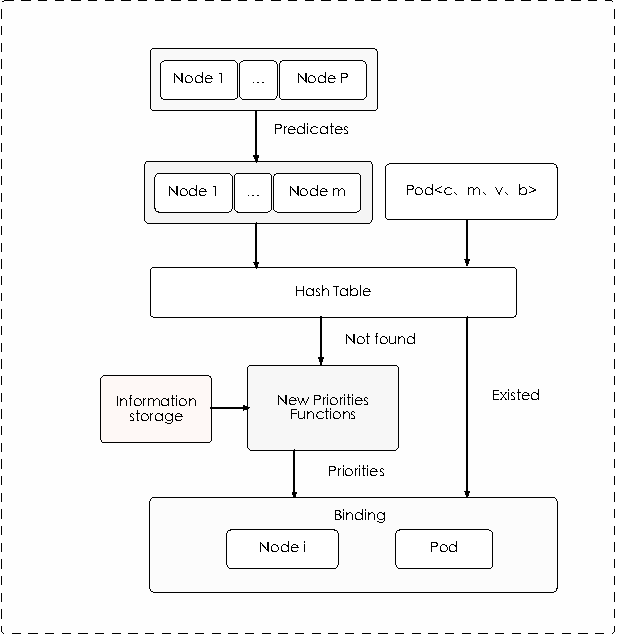
\includegraphics{scheduler-mrws}
	\caption{MRWS算法调度流程}
	\label{fig:xfig1}
\end{figure}


\subsection{插图}
\label{sec:graphs}

强烈推荐《\LaTeXe\ 插图指南》!关于子图形的使用细节请参看 \pkg{subcaption} 宏包的说明文档。

\subsubsection{一个图形}
\label{sec:onefig}
一般图形都是处在浮动环境中。之所以称为浮动是指最终排版效果图形的位置不一定与源文
件中的位置对应\footnote{This is not a bug, but a feature of \LaTeX!},这也是刚使
用 \LaTeX{} 同学可能遇到的问题。如果要强制固定浮动图形的位置,请使用 \pkg{float} 宏包,
它提供了 \texttt{[H]} 参数,比如图~\ref{fig:xfig1}。
\begin{figure}[H] % use float package if you want it here
  \centering
  
\includegraphics{thu-whole-logo}
  \caption{利用 Xfig 制图}
  \label{fig:xfig1}
\end{figure}

大学之道,在明明德,在亲民,在止于至善。知止而后有定;定而后能静;静而后能安;安
而后能虑;虑而后能得。物有本末,事有终始。知所先后,则近道矣。古之欲明明德于天
下者,先治其国;欲治其国者,先齐其家;欲齐其家者,先修其身;欲修其身者,先正其心;
欲正其心者,先诚其意;欲诚其意者,先致其知;致知在格物。物格而后知至;知至而后
意诚;意诚而后心正;心正而后身 修;身修而后家齐;家齐而后国治;国治而后天下
平。自天子以至于庶人,壹是皆以修身为本。其本乱而未治者 否矣。其所厚者薄,而其所
薄者厚,未之有也!

\hfill —— 《大学》


\subsubsection{多个图形}
\label{sec:multifig}

如果多个图形相互独立,并不共用一个图形计数器,那么
用 \texttt{minipage} 或者\texttt{parbox} 就可以。否则,请参看
图~\ref{fig:big1-subcaptionbox},它包含两个小图,分别是图~\ref{fig:subfig1}和
图~\ref{fig:subfig2}。推荐使用 \cs{subcaptionbox},因为可以像
图~\ref{fig:big1-subcaptionbox} 那样对齐子图的标题,也可以使用 \pkg{subcaption}
宏包的 \cs{subcaption}(放在 minipage中,用法同\cs{caption})或
是 \pkg{subfigure} 、\pkg{subtable}环境,像图~\ref{fig:big1-subfigure},不要再
用 \cs{subfloat}、\cs{subfigure} 和 \cs{subtable}。

\begin{figure}[h]
  \centering%
  \subcaptionbox{第一个小图形\label{fig:subfig1}}[3cm] %标题的长度,超过则会换行,如下一个小图。
    {
\includegraphics[height=3cm]{thu-fig-logo}}%
  \hspace{4em}%
  \subcaptionbox{第二个小图形,注意这个图略矮些。如果标题很长的话,它会自动换行\label{fig:subfig2}}
      {
\includegraphics[height=2cm]{thu-text-logo}}
  \caption{包含子图形的大图形(subcaptionbox示例)}
  \label{fig:big1-subcaptionbox}
\end{figure}
\begin{figure}[h]
  \centering%
  \begin{subfigure}{3cm}
    
\includegraphics[height=3cm]{thu-fig-logo}
    \caption{第一个小图形}
  \end{subfigure}%
  \hspace{4em}%
  \begin{subfigure}{0.5\textwidth}
    
\includegraphics[height=2cm]{thu-text-logo}
    \caption{第二个小图形,注意这个图略矮些。subfigure中同一行的子图在顶端对齐。}
  \end{subfigure}
  \caption{包含子图形的大图形(subfigure示例)}
  \label{fig:big1-subfigure}
\end{figure}

古之学者必有师。师者,所以传道受业解惑也。人非生而知之者,孰能无惑?惑而不从师,
其为惑也,终不解矣。生乎吾前,其闻道也固先乎吾,吾从而师之;生乎吾後,其闻道也亦
先乎吾,吾从而师之。吾师道也,夫庸知其年之先後生於吾乎!是故无贵无贱无长无少,道
之所存,师之所存也。

嗟乎!师道之不传也久矣,欲人之无惑也难矣。古之圣人,其出人也远矣,犹且从师而问焉;
今之众人,其下圣人也亦远矣,而耻学於师。是故圣益圣,愚益愚。圣人之所以为圣,愚
人之所以为愚,其皆出於此乎?爱其子,择师而教之,於其身也,则耻师焉,惑焉。彼童子
之师,授之书而习其句读者,非吾所谓传其道、解其惑者也。句读之不知,惑之不解,或师
焉,或不焉,小学而大遗,吾未见其明也。巫医、乐师、百工之人不耻相师,  士大夫之族
曰“师”曰“弟子”之云者,则群聚而笑之。问之,则曰:彼与彼年相若也,道相似也,位
卑则足羞,官盛则近谀。呜呼!师道之不复,可知矣。巫医、乐师、百工之人。吾子不齿,
今其智乃反不能及,其可怪也欤!圣人无常师。孔子师郯子、苌子、师襄、老聃。郯子之徒,
其贤不及孔子。孔子曰:“三人行,必有我师。”是故弟子不必不如师,师不必贤於弟子。
闻道有先後,术业有专攻,如是而已。

如果要把编号的两个图形并排,那么小页就非常有用了:
\begin{figure}
\begin{minipage}{0.48\textwidth}
  \centering
  
\includegraphics[height=2cm]{thu-whole-logo}
  \caption{并排第一个图}
  \label{fig:parallel1}
\end{minipage}\hfill
\begin{minipage}{0.48\textwidth}
  \centering
  
\includegraphics[height=2cm]{thu-whole-logo}
  \caption{并排第二个图}
  \label{fig:parallel2}
\end{minipage}
\end{figure}

李氏子蟠,年十七,好古文、六艺,经传皆通习之,不拘於时,学於余。余嘉其能行古
道,作师说以贻之。

\hfill —— 韩愈(唐)
